\documentclass{standalone}
\usepackage{tikz}
\usetikzlibrary{patterns, positioning}

\begin{document}
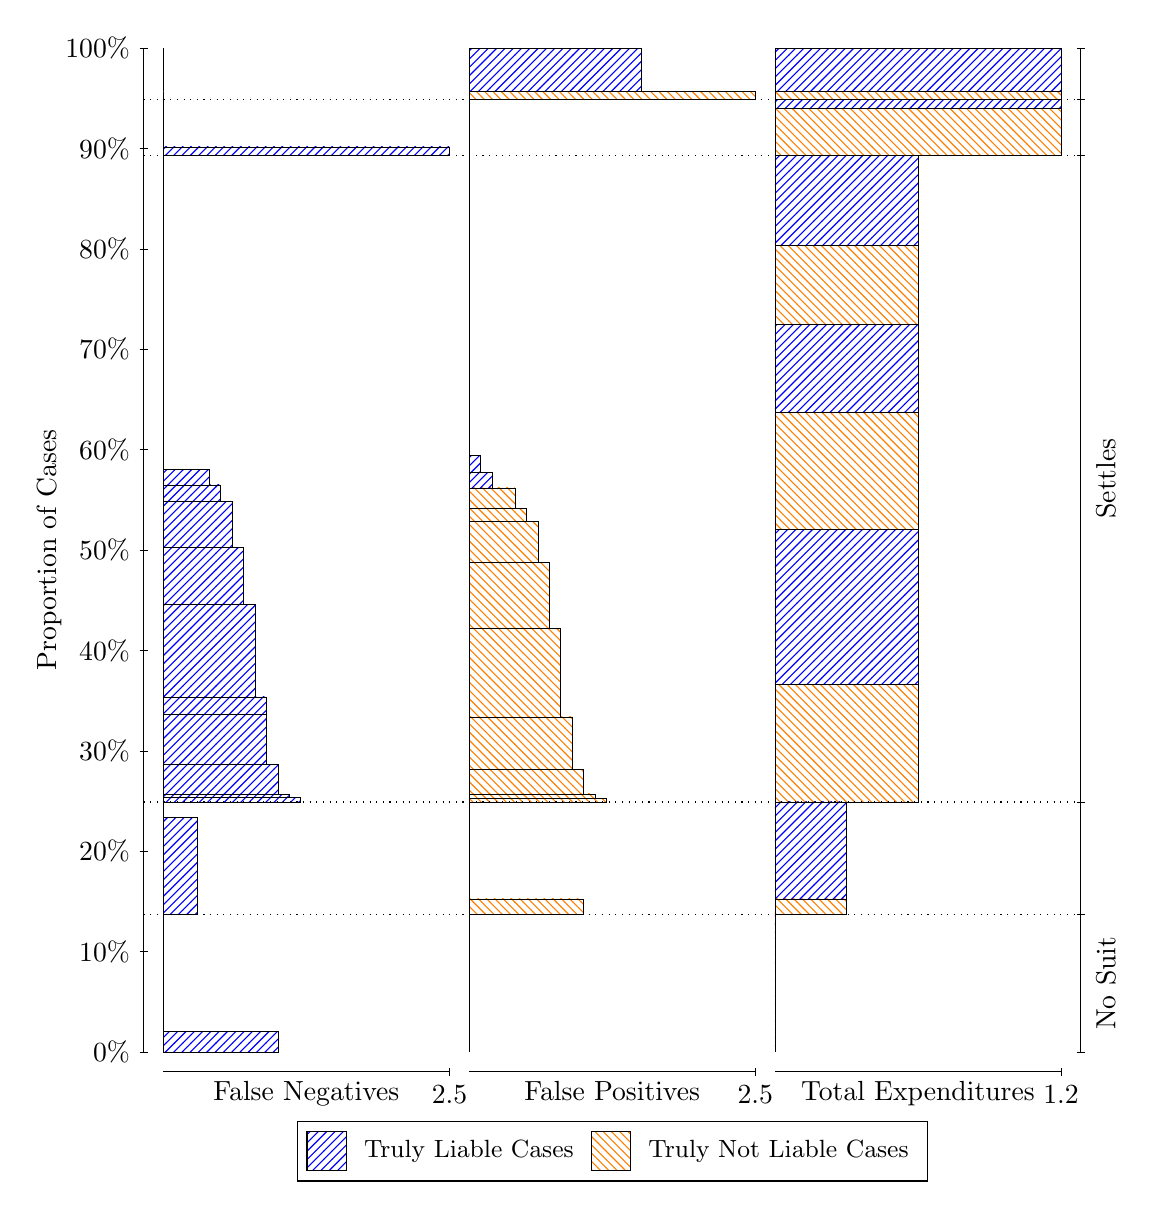
\begin{tikzpicture}
\draw[black, very thin] (1.5,1.75) -- (1.5,14.5);
\node[rotate=90, anchor=center] at (0.3, 8.125) {Proportion of Cases};
\draw[black, very thin] (1.45,1.75) -- (1.55,1.75);
\node[anchor=east] at (1.45, 1.75) {0\%};
\draw[black, very thin] (1.45,3.025) -- (1.55,3.025);
\node[anchor=east] at (1.45, 3.025) {10\%};
\draw[black, very thin] (1.45,4.3) -- (1.55,4.3);
\node[anchor=east] at (1.45, 4.3) {20\%};
\draw[black, very thin] (1.45,5.575) -- (1.55,5.575);
\node[anchor=east] at (1.45, 5.575) {30\%};
\draw[black, very thin] (1.45,6.85) -- (1.55,6.85);
\node[anchor=east] at (1.45, 6.85) {40\%};
\draw[black, very thin] (1.45,8.125) -- (1.55,8.125);
\node[anchor=east] at (1.45, 8.125) {50\%};
\draw[black, very thin] (1.45,9.4) -- (1.55,9.4);
\node[anchor=east] at (1.45, 9.4) {60\%};
\draw[black, very thin] (1.45,10.675) -- (1.55,10.675);
\node[anchor=east] at (1.45, 10.675) {70\%};
\draw[black, very thin] (1.45,11.95) -- (1.55,11.95);
\node[anchor=east] at (1.45, 11.95) {80\%};
\draw[black, very thin] (1.45,13.225) -- (1.55,13.225);
\node[anchor=east] at (1.45, 13.225) {90\%};
\draw[black, very thin] (1.45,14.5) -- (1.55,14.5);
\node[anchor=east] at (1.45, 14.5) {100\%};

\draw[black, very thin] (13.4,1.75) -- (13.4,14.5);
\draw[black, very thin] (13.35,1.75) -- (13.45,1.75);
\node[anchor=west] at (13.35, 1.75) {};
\draw[black, very thin] (13.35,3.495) -- (13.45,3.495);
\node[anchor=west] at (13.35, 3.495) {};
\draw[black, very thin] (13.35,4.9247) -- (13.45,4.9247);
\node[anchor=west] at (13.35, 4.9247) {};
\draw[black, very thin] (13.35,13.14) -- (13.45,13.14);
\node[anchor=west] at (13.35, 13.14) {};
\draw[black, very thin] (13.35,13.843) -- (13.45,13.843);
\node[anchor=west] at (13.35, 13.843) {};
\draw[black, very thin] (13.35,14.5) -- (13.45,14.5);
\node[anchor=west] at (13.35, 14.5) {};

\draw[black, very thin, pattern color=blue, pattern=north east lines] (1.75,1.75) rectangle (3.2033,2.0113);
\draw[black, very thin, pattern color=orange, pattern=north west lines] (1.75,2.0113) rectangle (1.75,3.495);
\draw[black, very thin, pattern color=blue, pattern=north east lines] (1.75,3.495) rectangle (2.186,4.7254);
\draw[black, very thin, pattern color=orange, pattern=north west lines] (1.75,4.7254) rectangle (1.75,4.9247);
\draw[black, very thin, pattern color=blue, pattern=north east lines] (1.75,4.9247) rectangle (3.494,4.9794);
\draw[black, very thin, pattern color=blue, pattern=north east lines] (1.75,4.9794) rectangle (3.3487,5.0199);
\draw[black, very thin, pattern color=blue, pattern=north east lines] (1.75,5.0199) rectangle (3.2033,5.3976);
\draw[black, very thin, pattern color=blue, pattern=north east lines] (1.75,5.3976) rectangle (3.058,6.0402);
\draw[black, very thin, pattern color=blue, pattern=north east lines] (1.75,6.0402) rectangle (3.058,6.2608);
\draw[black, very thin, pattern color=blue, pattern=north east lines] (1.75,6.2608) rectangle (2.9127,7.4375);
\draw[black, very thin, pattern color=blue, pattern=north east lines] (1.75,7.4375) rectangle (2.7673,8.1623);
\draw[black, very thin, pattern color=blue, pattern=north east lines] (1.75,8.1623) rectangle (2.622,8.7389);
\draw[black, very thin, pattern color=blue, pattern=north east lines] (1.75,8.7389) rectangle (2.4767,8.9507);
\draw[black, very thin, pattern color=blue, pattern=north east lines] (1.75,8.9507) rectangle (2.3313,9.1505);
\draw[black, very thin, pattern color=orange, pattern=north west lines] (1.75,9.1505) rectangle (1.75,13.14);
\draw[black, very thin, pattern color=blue, pattern=north east lines] (1.75,13.14) rectangle (5.3833,13.245);
\draw[black, very thin, pattern color=orange, pattern=north west lines] (1.75,13.245) rectangle (1.75,13.843);
\draw[black, very thin, pattern color=orange, pattern=north west lines] (1.75,13.843) rectangle (1.75,13.948);
\draw[black, very thin, pattern color=blue, pattern=north east lines] (1.75,13.948) rectangle (1.75,14.5);
\draw[black, very thin, pattern color=orange, pattern=north west lines] (5.6333,1.75) rectangle (5.6333,3.2337);
\draw[black, very thin, pattern color=blue, pattern=north east lines] (5.6333,3.2337) rectangle (5.6333,3.495);
\draw[black, very thin, pattern color=orange, pattern=north west lines] (5.6333,3.495) rectangle (7.0867,3.6943);
\draw[black, very thin, pattern color=blue, pattern=north east lines] (5.6333,3.6943) rectangle (5.6333,4.9247);
\draw[black, very thin, pattern color=orange, pattern=north west lines] (5.6333,4.9247) rectangle (7.3773,4.9747);
\draw[black, very thin, pattern color=orange, pattern=north west lines] (5.6333,4.9747) rectangle (7.232,5.0266);
\draw[black, very thin, pattern color=orange, pattern=north west lines] (5.6333,5.0266) rectangle (7.0867,5.3422);
\draw[black, very thin, pattern color=orange, pattern=north west lines] (5.6333,5.3422) rectangle (6.9413,6.0058);
\draw[black, very thin, pattern color=orange, pattern=north west lines] (5.6333,6.0058) rectangle (6.796,7.133);
\draw[black, very thin, pattern color=orange, pattern=north west lines] (5.6333,7.133) rectangle (6.6507,7.971);
\draw[black, very thin, pattern color=orange, pattern=north west lines] (5.6333,7.971) rectangle (6.5053,8.4911);
\draw[black, very thin, pattern color=orange, pattern=north west lines] (5.6333,8.4911) rectangle (6.36,8.6564);
\draw[black, very thin, pattern color=orange, pattern=north west lines] (5.6333,8.6564) rectangle (6.2147,8.9141);
\draw[black, very thin, pattern color=blue, pattern=north east lines] (5.6333,8.9141) rectangle (5.924,9.1138);
\draw[black, very thin, pattern color=blue, pattern=north east lines] (5.6333,9.1138) rectangle (5.7787,9.3257);
\draw[black, very thin, pattern color=blue, pattern=north east lines] (5.6333,9.3257) rectangle (5.6333,13.14);
\draw[black, very thin, pattern color=orange, pattern=north west lines] (5.6333,13.14) rectangle (5.6333,13.738);
\draw[black, very thin, pattern color=blue, pattern=north east lines] (5.6333,13.738) rectangle (5.6333,13.843);
\draw[black, very thin, pattern color=orange, pattern=north west lines] (5.6333,13.843) rectangle (9.2667,13.948);
\draw[black, very thin, pattern color=blue, pattern=north east lines] (5.6333,13.948) rectangle (7.8133,14.5);
\draw[black, very thin, pattern color=orange, pattern=north west lines] (9.5167,1.75) rectangle (9.5167,3.2337);
\draw[black, very thin, pattern color=blue, pattern=north east lines] (9.5167,3.2337) rectangle (9.5167,3.495);
\draw[black, very thin, pattern color=orange, pattern=north west lines] (9.5167,3.495) rectangle (10.425,3.6943);
\draw[black, very thin, pattern color=blue, pattern=north east lines] (9.5167,3.6943) rectangle (10.425,4.9247);
\draw[black, very thin, pattern color=orange, pattern=north west lines] (9.5167,4.9247) rectangle (11.333,6.4194);
\draw[black, very thin, pattern color=blue, pattern=north east lines] (9.5167,6.4194) rectangle (11.333,8.3845);
\draw[black, very thin, pattern color=orange, pattern=north west lines] (9.5167,8.3845) rectangle (11.333,9.8743);
\draw[black, very thin, pattern color=blue, pattern=north east lines] (9.5167,9.8743) rectangle (11.333,10.99);
\draw[black, very thin, pattern color=orange, pattern=north west lines] (9.5167,10.99) rectangle (11.333,11.995);
\draw[black, very thin, pattern color=blue, pattern=north east lines] (9.5167,11.995) rectangle (11.333,13.14);
\draw[black, very thin, pattern color=orange, pattern=north west lines] (9.5167,13.14) rectangle (13.15,13.738);
\draw[black, very thin, pattern color=blue, pattern=north east lines] (9.5167,13.738) rectangle (13.15,13.843);
\draw[black, very thin, pattern color=orange, pattern=north west lines] (9.5167,13.843) rectangle (13.15,13.948);
\draw[black, very thin, pattern color=blue, pattern=north east lines] (9.5167,13.948) rectangle (13.15,14.5);
\draw[black, dotted] (1.5,3.495) -- (13.4,3.495);
\draw[black, dotted] (1.5,4.9247) -- (13.4,4.9247);
\draw[black, dotted] (1.5,13.14) -- (13.4,13.14);
\draw[black, dotted] (1.5,13.843) -- (13.4,13.843);
\draw[black, very thin] (1.75,1.5) -- (5.3833,1.5);
\node[anchor=north] at (3.5667, 1.5) {False Negatives};
\draw[black, very thin] (5.3833,1.45) -- (5.3833,1.55);
\node[anchor=north] at (5.3833, 1.45) {2.5};

\draw[black, very thin] (5.6333,1.5) -- (9.2667,1.5);
\node[anchor=north] at (7.45, 1.5) {False Positives};
\draw[black, very thin] (9.2667,1.45) -- (9.2667,1.55);
\node[anchor=north] at (9.2667, 1.45) {2.5};

\draw[black, very thin] (9.5167,1.5) -- (13.15,1.5);
\node[anchor=north] at (11.333, 1.5) {Total Expenditures};
\draw[black, very thin] (13.15,1.45) -- (13.15,1.55);
\node[anchor=north] at (13.15, 1.45) {1.2};

\node[black, centered, rotate=90] at (13.72, 2.6225) {No Suit};

\node[black, centered, rotate=90] at (13.72, 9.0323) {Settles};



\draw (7.449999999999999,1.5) node[draw=none] (baseCoordinate) {};
\begin{scope}[align=center]
        \matrix[scale=0.5, draw=black, below=0.5cm of baseCoordinate, nodes={draw}, column sep=0.1cm]{
            \node[rectangle, draw, minimum width=0.5cm, minimum height=0.5cm, pattern=north east lines, pattern color=blue] {}; &
            \node[draw=none, font=\small] (B) {Truly Liable Cases}; &
            \node[rectangle, draw, minimum width=0.5cm, minimum height=0.5cm, pattern=north west lines, pattern color=orange] {}; &
            \node[draw=none, font=\small] (B) {Truly Not Liable Cases}; \\
            };
\end{scope}

\end{tikzpicture}
\end{document}